\chapter{Implementacija i korisničko sučelje}
		
		
		\section{Korištene tehnologije i alati}
		
			
			
			Članovi unutar tima su komunicirali koristeći aplikaciju Discord. 
			Za izradu UML dijagrama koristen je alat Astah Professional
			, a kao sustav za upravljanje
			izvornim kodom Git. Udaljeni repozitorij projekta je dostupan na web platformi
			GitLab. Od razvojnih okruženja smo koristili Microsoft Visual Studio Code i Sublime Text 3. Svi djelovi aplikacije su ostvareni korištenjem programskog jezika JavaScript. Za izradu frontenda koristena je biblioteka ReactJs. Održavana je od strane Facebooka. React se najčešće koristi kao osnova  u razvoju web ili mobilnih aplikacija. Za backend je korišten Next.js framework kreirao od strane Vercela. Next.js se koristi za "server-side rendering" i generiranje statičkih stranica. Za prikaz podataka na karti koristili smo Google Maps api. Dizajn je ostvaren koristeći web aplikaciju Figma koja služi za dizajn korisnićkih sučelja. Bazu podataka smo napravili koristeći Firebase, koji služi za izradu NoSql baza i održava ga Google. Za pisanje dokumentacije korištena je web aplikacija Overleaf.
            \eject 
			
	
		\section{Ispitivanje programskog rješenja}
			
			\textbf{\textit{dio 2. revizije}}\\
			
			 \textit{U ovom poglavlju je potrebno opisati provedbu ispitivanja implementiranih funkcionalnosti na razini komponenti i na razini cijelog sustava s prikazom odabranih ispitnih slučajeva. Studenti trebaju ispitati temeljnu funkcionalnost i rubne uvjete.}
	
			
			\subsection{Ispitivanje komponenti}
			\textit{Potrebno je provesti ispitivanje jedinica (engl. unit testing) nad razredima koji implementiraju temeljne funkcionalnosti. Razraditi \textbf{minimalno 6 ispitnih slučajeva} u kojima će se ispitati redovni slučajevi, rubni uvjeti te izazivanje pogreške (engl. exception throwing). Poželjno je stvoriti i ispitni slučaj koji koristi funkcionalnosti koje nisu implementirane. Potrebno je priložiti izvorni kôd svih ispitnih slučajeva te prikaz rezultata izvođenja ispita u razvojnom okruženju (prolaz/pad ispita). }
			
			
			
			\subsection{Ispitivanje sustava}



    \textbf{Ispitni slučaj 1: Uspješna prijava korisnika}
    Prijavljujemo se kao već registrirani korisnik sa točnim podatcima. 
    
    Rezultat: Uspješna prijava

    \begin{figure}[H]
			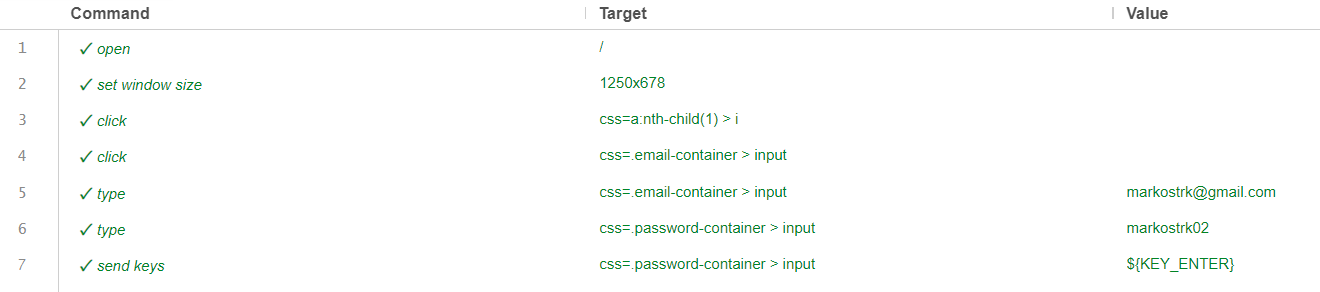
\includegraphics[scale=0.5]{slike/UspjesnaPrijava1.png}
			\centering
			\caption{Selenium Uspješna prijava}
			\label{fig:promjene}
		          \end{figure}


\begin{figure}[H]
			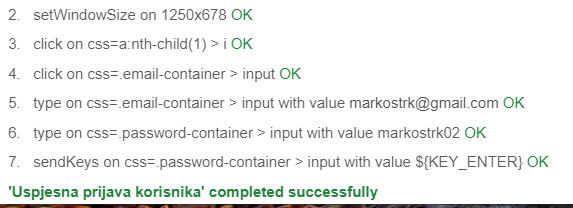
\includegraphics[scale=0.8]{slike/UspjesnaPrijava2.png}
			\centering
			\caption{Selenium Uspješna prijava - log}
			\label{fig:promjene}
		          \end{figure}
    



    \textbf{Ispitni slučaj 2: Neuspješna prijava korisnika}
    Prijavljujemo se kao već registrirani korisnik sa netočnim podatcima. 
    
    Rezultat: Neuspješna prijava - vraćanje na početnu stranicu

    \begin{figure}[H]
			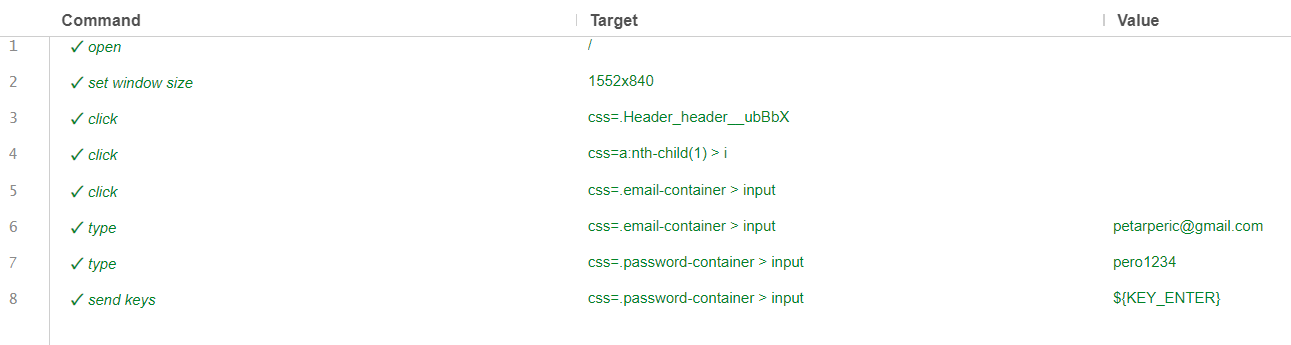
\includegraphics[scale=0.5]{slike/NeuspjesnaPrijava1.png}
			\centering
			\caption{Selenium Neuspješna prijava}
			\label{fig:promjene}
		          \end{figure}


\begin{figure}[H]
			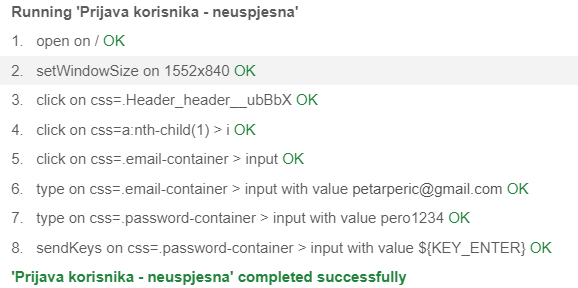
\includegraphics[scale=0.8]{slike/NeuspjesnaPrijava2.png}
			\centering
			\caption{Selenium Neuspješna prijava - log}
			\label{fig:promjene}
		          \end{figure}

    \textbf{Ispitni slučaj 3: Uspješna registracija privatnog korisnika}
    Popunjavamo obrazac za registraciju sa ispravnim podatcima.
    
    Rezultat: Uspještna registracija korisnika

    \begin{figure}[H]
			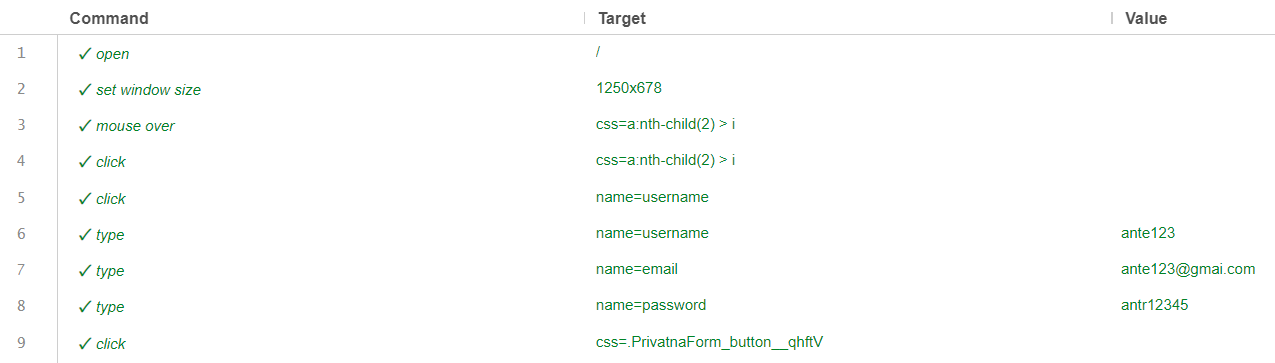
\includegraphics[scale=0.5]{slike/UspjesnaRegistracija1.png}
			\centering
			\caption{Selenium Uspješna Registracija}
			\label{fig:promjene}
		          \end{figure}


\begin{figure}[H]
			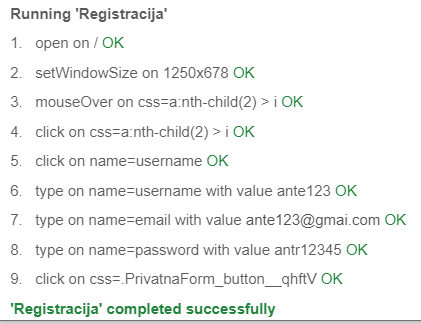
\includegraphics[scale=0.8]{slike/UspjesnaRegistracija2.png}
			\centering
			\caption{Selenium Uspješna registracija - log}
			\label{fig:promjene}
		          \end{figure}

            \textbf{Ispitni slučaj 4: Neuspješna registracija privatnog korisnika}
    Popunjavamo obrazac za registraciju sa neispravnim podatcima.
    
    Rezultat: Sustav javlja pogrešku, te nam nudi ponovni upis novih podataka

    \begin{figure}[H]
			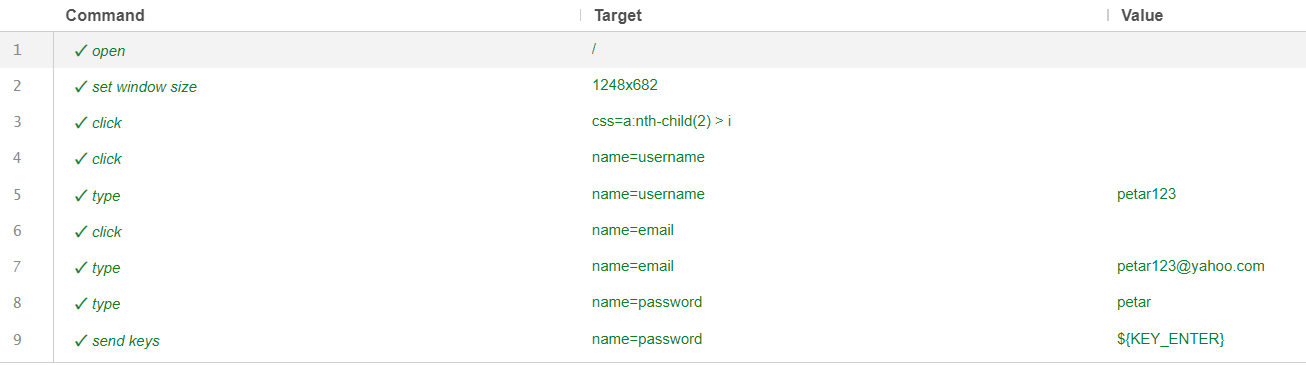
\includegraphics[scale=0.5]{slike/NeuspjesnaRegistracija2.png}
			\centering
			\caption{Selenium Neuspješna Registracija}
			\label{fig:promjene}
		          \end{figure}


\begin{figure}[H]
			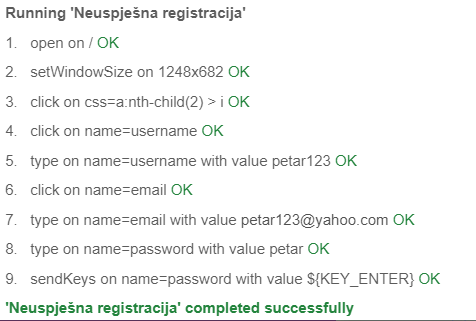
\includegraphics[scale=0.8]{slike/NeuspjesnaRegistracija1.png}
			\centering
			\caption{Selenium Neupješna registracija - log}
			\label{fig:promjene}
		          \end{figure}
    
			
			\eject 
		
		
		\section{Dijagram razmještaja}


            Dijagrami razmještaja opisuju topologiju sklopovlja i programsku potporu koja se koristi u implementaciji sustava  u njegovom radnom okruženju. Na jednom poslužiteljskom računalu nalazi se web poslužitelj, a na drugom poslužitelj baze podataka. Klijenti koriste web preglednik kako bi pristupili web aplikaciji. Sustav je baziran na arhitekturi klijent - poslužitelj, a komunikacija između računala korisnika i poslužitelja odvija se preko HTTP veze. 
            
			\begin{figure}[H]
			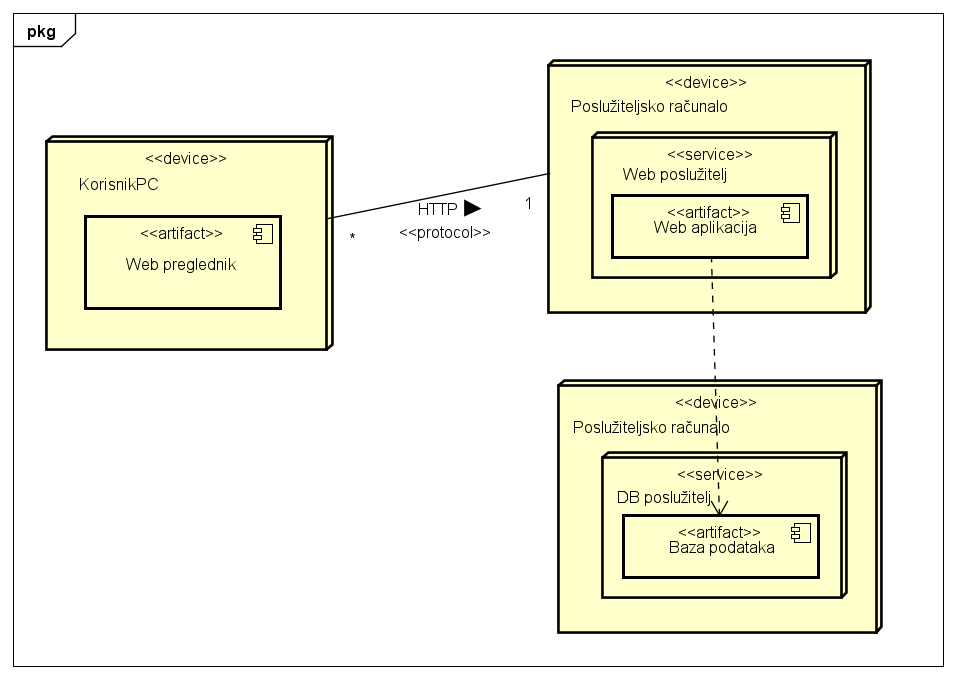
\includegraphics[scale=0.7]{slike/DijagramRazmjestaja.png}
			\centering
			\caption{Dijagram razmještaja}
			\label{fig:promjene}
				\end{figure}
			
			\eject 
		
		\section{Upute za puštanje u pogon}
		

   \textbf{Baza podataka}

    Za bazu podataka koristili smo Googleov \href{https://firebase.google.com/}{Firebase} u koji se prijavljujemo koristeći google račun progi.dogfriendly@gmail.com. Nakon prijave imamo pristup svim podatcima u bazi podataka. Možemo vidjeti sve tablice (collection), uređivati ih, dodavati/brisati nove podatke

    \textbf{Hoasting aplikacije}
    
    Za hostanje aplikacije koristili smo \href{https://vercel.com/}{Vercel}. To je platforma koja nam omogućuje jednostavno i besplatno povezivanje sa Gitlab računom i hostanje aplikacije. Potrebno je samo povezati gitlab račun te odabrati ime web stranice. 
			
			
			\eject 